% TODO:
% * obrázek s chomského hierarchií
% * obrázek se všemi důležitými modely
% * Kasai
%%%%%%%%%%%%%%%%%%%%%%%%%%%%%%%%%%%%%%%%%%%%%%%%%%%%%%%%%%%%%%%%%%%%%%%%%%
\chapter{Pojmy a definice}

V~této kapitole zavádím a definuji pojmy, ze kterých vycházím v~dalších částech své práce. Ve stručnosti se zabývám problematikou řízených gramatik a definuji programové a stavové gramatiky. Dále uvádím definici hlubokého zásobníkového automatu a jeho konečné varianty. Nakonec zařazuji jazyky přijímané těmito automaty spolu s~jazyky generovanými řízenými gramatikami do kontextu označovaném jako hierarchie mezi kontextovými a bezkontextovými jazyky.

%=========================================================================
\section{Základní pojmy}

V~této práci předpokládám základní znalosti z~teorie formálních jazyků. Dále zavádím následující konvence.

\emph{Abeceda} je konečná neprázdná množina symbolů. 
\emph{Prázdný řetězec} se značí symbolem $\varepsilon$. 
Nechť $\Sigma$ je abeceda, pak $\varepsilon$ je \emph{řetězec} nad abecedou $\Sigma$, a pokud $x$ je řetězec nad $\Sigma$ a $a \in \Sigma$, pak $xa$ je řetězec na abecedou $\Sigma$.  
$\Sigma^*$ je množina všech řetězců nad $\Sigma$ a $\Sigma^+ = \Sigma^* - \{\varepsilon\}$. 
Pro řetězec $v \in \Sigma$ platí, že $|v|$ označuje délku řetězce $v$ a $\mathrm{alph}(v)$ značí množinu symbolů vyskytujících se v~řetězci $v$. Pokud V~je množina symbolů, pak $\mathrm{occur}(v, V)$ značí počet výskytů symbolů z~$V$ v~řetězci $v$. 
Nechť $I$ je podmnožina celých čísel, pak $\mathrm{max}(I)$ označuje největší číslo v~$I$.

%=========================================================================
\section{Hluboké zásobníkové automaty}

Zásobníkový automat je modelem pro bezkontextové jazyky. Umožňuje přepisovat symbol na vrcholu zásobníku za řetězec. Meduna tento automat zobecnil a zvýšil jeho sílu tak, že lze přepisovat libovolný symbol na zásobníku. Tyto automaty se označují jako \emph{hluboké zásobníkové automaty}. 

% DEFINICE: DEEP PDA

\begin{Def} \label{def_deep_pda}
\emph{Hluboký zásobníkový automat} je dle \cite{Meduna:DeepPDA} definován jako uspořádaná sedmice $M = (Q,\Sigma,\Gamma, R, s, S, F)$, kde 

\begin{description*}
\item  $Q$ je konečná množina stavů, 
\item  $\Sigma$ vstupní abeceda, 
\item  $\Gamma$ zásobníková abeceda, přičemž $\Sigma \subseteq \Gamma$ a $Q \cap \Gamma = \emptyset$,
\item  $R$ je konečná množina pravidel typu $(m, q, A, p, v) \in (\{1,2,3,\dots\} \times Q \times (\Gamma-\Sigma)\times   Q \times {\Gamma}^+)$, píšeme $mqA \rightarrow pv$,
\item  $s \in Q$ je počáteční stav, 
\item  $S \in \Gamma$ počáteční zásobníkový symbol, 
\item  $F \subseteq Q$ je množina koncových stavů.
\end{description*}

%% Definice konfigurace, derivace
\emph{Konfigurace} automatu $M$ je prvek z~množiny $(Q \times \Sigma^* \times \Gamma^*)$. 
Nechť $X$, $Y$ jsou dvě konfigurace. 
$M$ přečte symbol na vstupní pásce a přejde z~$X$ do $Y$, tzv. \emph{pop operace}, píšeme $X$  ${}_p{\Rightarrow}$  $Y$ $[mqA \rightarrow pv]$, zjednodušeně $X$  ${}_p{\Rightarrow}$  $Y$, pokud $X = (q, au, az)$, $Y = (q, u, z)$, kde $q \in Q$, $a \in \Sigma$, $u \in \Sigma^*$, $z \in \Gamma^*$.
$M$ přepíše symbol na zásobníku a přejde z~$X$ do $Y$, tzv. \emph{expanze}, píšeme $X$  ${}_e{\Rightarrow}$  $Y$ $[mqA \rightarrow pv]$, zjednodušeně $X$  ${}_e{\Rightarrow}$  $Y$, pokud $X = (q, w, uAz)$, $Y = (p, w, uvz)$, $mqA \rightarrow pv \in R$ a platí $\mathrm{occur}(u,\Gamma - \Sigma) = m - 1 $, kde $p$, $q \in Q$, $w \in \Sigma^*$, $A \in \Gamma$, $u$, $v$, $z \in \Gamma^*$. 
$M$ provede \emph{přechod} z~$X$ do $Y$, píšeme $X$  ${\Rightarrow}$  $Y$ $[mqA \rightarrow pv]$, zjednodušeně $X$  ${\Rightarrow}$  $Y$, pokud provede expanzi, nebo operaci pop.


\begin{figure}[ht]
\centering
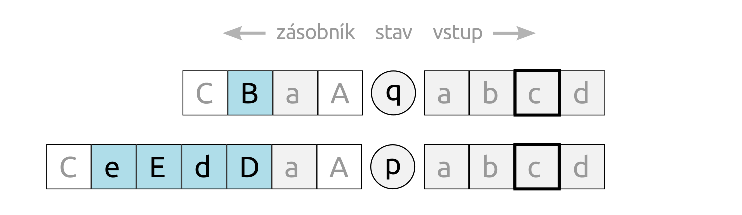
\includegraphics{img/bp_pda01.eps} \bigskip \\
\caption{Aplikace pravidla $2 q B \rightarrow p DdEe$ v~hlubokém zásobníkovém automatu .}
\end{figure}


%% sekvence přechodů
Nechť $X$ je konfigurace. $M$ provede \emph{nula přechodů} z~$X$ do $X$, píšeme $X \Rightarrow^0 X [\varepsilon]$, zjednodušeně $X \Rightarrow^0 X$. Nechť $X_0, X_1, X_2,\dots,X_n $ je sekvence přechodů konfigurací pro $n \ge 1$  a $X_{i-1} \Rightarrow X_i [r_i]$, kde $r_i \in R$, pro každé $i \in \{1, 2, 3,\dots, n\}$, tedy platí $X_0 \Rightarrow X_1 [r_1] \Rightarrow X_2 [r_2] \dots \Rightarrow X_n [r_n]$. Pak $M$ provede \emph{$n$ přechodů} z~$X_0$ do $X_n$. Píšeme $X_{0} \Rightarrow^n X_n [r_1 \dots r_n]$, zjednodušeně $X_{0} \Rightarrow^n X_n$. Pokud $X_{0} \Rightarrow^n X_n [r_1 \dots r_n]$ pro nějaké $n \ge 1$, pak $X_{0} \Rightarrow^+ X_n [r_1 \dots r_n]$. Pokud $X_{0} \Rightarrow^n X_n [r_1 \dots r_n]$ pro nějaké $n \ge 0$, pak $X_{0} \Rightarrow^* X_n [r_1 \dots r_n]$.

% Hloubka a jazyk
Říkáme, že pravidlo $mqA \rightarrow pv \in R$ je hloubky $m$. Pokud existuje nejmenší přirozené číslo $n$ takové, že každé pravidlo v~$M$ je hloubky menší nebo rovno $n$, říkáme, že $M$ je hloubky $n$, píšeme ${}_nM$. Jazyk přijímaný automatem ${}_nM$ je
    $$L({}_nM) = \{ w \in \Sigma^* \mid (s,w,S) \Rightarrow^* (f, \varepsilon, \varepsilon)\textnormal{, kde }f \in F \}.$$


\end{Def}

\begin{figure}[ht]
\centering
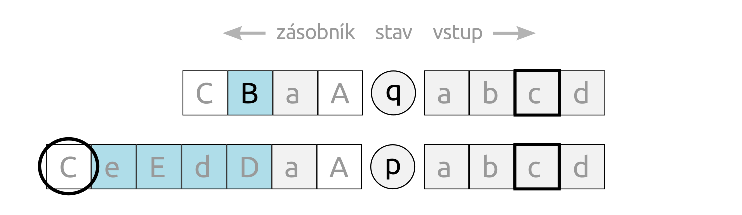
\includegraphics{img/bp_pda02.eps} \bigskip \\
\caption{V~hlubokém zásobníkovém automatu indexu 3 nelze pravidlo $2 q B \rightarrow p DdEe$ v~aktuální konfiguraci aplikovat.}
\end{figure}

% DEFINICE: FINITELY EXPANDABLE DEEP PDA

\begin{Def} Podle \cite{Meduna:FinitelyDeepPDA} je \emph{hluboký zásobníkový automat konečného indexu} uspořádaná osmice $M_n = (Q,\Sigma,\Gamma, R, s, S, F, n)$, jehož definice vychází z~hlubokého zásobníkového automatu. Symbol $n \in \{1,2,3,\dots\}$ označuje maximální počet nevstupních symbolů, které mohou být uložené na zásobníku. Expanze $X$  ${}_e{\Rightarrow}$  $Y$ může proběhnout jen v~případě, že v~konfiguraci $Y$ bude na zásobníku $n$ a méně nevstupních symbolů.  O~hloubce zásobníku tohoto typu automatu se předpokládá, že je rozšiřitelná tak, aby zásobník mohl přijmout až $n$ nevstupních symbolů.

%% Definovat krok, derivaci a jazyk

\end{Def}

%=========================================================================
\section{Řízené gramatiky}

Řízené gramatiky vycházejí z~definice bezkontextové gramatiky. Zachovává se základní tvar pravidla, ale mění se způsob derivace. Tímto způsobem lze zvýšit mocnost modelu bez zbytečného komplikování pravidel \cite{Krivka}. Mezi řízené gramatiky patří například programové, maticové a stavové.  

% DEFINICE: BEZKONTEXTOVE GRAMATIKY
\begin{Def}\label{def_bezkontext_gram}

\emph{Bezkontextová gramatika} \cite{Krivka:RewritingSystems} je čtveřice $G = (V,T,P,S)$, kde 
\begin{description*}
\item $V = T \cup N$ je úplná abeceda, 
\item $T$ je abeceda terminálů, 
\item $N$ je abeceda neterminálů, 
\item $S \in N$ je počáteční symbol, 
\item $P$ je konečná množina pravidel tvaru $A \rightarrow v$, kde $A \in N$, $v \in V^*$.
\end{description*}
Nechť $A \rightarrow v~\in P$, $A \in N$, $v$, $x$, $y \in V^*$, pak bezkontextová gramatika $G$ provede derivační krok z~$xAy$ do $xvy$, píšeme $xAy \Rightarrow xvy [A~\rightarrow v]$, zjednodušeně $xAy \Rightarrow xvy$. 
Nechť $r_1, r_2, \dots r_m \in P$ pro $m \ge 0$, pak $G$ může provést sekvenci kroků dle těchto pravidel, zápisem $x {\Rightarrow}^m y [r_1 r_2 \dots r_m]$. Píšeme ${\Rightarrow}^+$ pro libovolné $m > 0$ a ${\Rightarrow}^*$ pro $m \ge 0$. 

Bezkontextová gramatika $G$ generuje jazyk $L(G)$, pro který platí $$L(G) = \{w \in T^* | S~{\Rightarrow}^* w\}.$$ 

\end{Def}

% DEFINICE: PROGRAMOVA GRAMATIKA
\begin{Def}
\emph{Programová gramatika} \cite{Krivka:RewritingSystems} je čtveřice $G = (V,T,P,S)$, kde $V$, $T$ a $S$ jsou definované stejně jako v~bezkontextových gramatikách. $P$ je konečná množina pravidel tvaru $r \colon A~\rightarrow v, g(r)$, kde $r$ je označení pravidla, $A \rightarrow v$ je pravidlo bezkontextové gramatiky a $g(r)$ je množina značení těch pravidel, která mohou být provedena v~dalším derivačním kroku po aplikaci pravidla $r$.
\end{Def}

\begin{Def}
\emph{Programová gramatika konečného indexu $n$} \cite{Krivka:RewritingSystems} je programová gramatika $G = (V,T,P,S)$, pro jejíž každou větnou formu $w \in L(G)$ existuje taková posloupnost derivačních kroků, kde se v~žádném kroku nevyskytuje více než $n$ neterminálů.
\end{Def}

% DEFINICE: STAVOVA GRAMATIKA
\begin{Def} \label{def_state_gram}
\emph{Stavová gramatika} je dle \cite{Kasai:Hierarchy} šestice $G=(V,W,T,S,s,P)$, kde 
\begin{description*}
\item $V = T \cup N$ je úplná abeceda, 
\item $W$ je konečná množina stavů, 
\item $T$ je abeceda terminálů, 
\item $N$ je abeceda neterminálů, 
\item $S \in N$ je počáteční symbol, 
\item $s \in W$ je počáteční stav, 
\item $P$ je konečná relace $(W \times N) \times (W \times V^+)$, pravidla zapisujeme $(q,A) \rightarrow (p,v)$.
\end{description*}
Nechť $(q,A) \rightarrow (p,v) \in P$, $p$, $q \in W$, $A \in N$, $v$, $x$, $y \in V^*$, pak stavová gramatika $G$ provede derivační krok z~$xAy$ do $xvy$, píšeme $(q, xAy) \Rightarrow (p, xvy) [(q,A) \rightarrow (p,v)]$, zjednodušeně $xAy \Rightarrow xvy$, právě tehdy když 
   $$\{Z \mid (q,Z) \rightarrow (p',v') \in P \textnormal{, } Z~\in \mathrm{alph}(x) \cap N \textnormal{, } p' \in W \textnormal{, } v' \in V^* \} = \emptyset.$$ 
Gramatika $G$ generuje jazyk 
$$L(G) = \{w \in T^* | (s, S) {\Rightarrow}^* (p, w), p,q \in W \}.$$


\end{Def}

\begin{Def}
\emph{Stavová gramatika konečného indexu $n$} \cite{Kasai:Hierarchy} je stavová gramatika $G=(V,W,T,S,s,P)$, pro kterou platí, že derivační krok $(q, xAy) \Rightarrow (p, xvy)$ za pomoci pravidla $(q,A) \rightarrow (p,v) \in P$, kde $p$, $q \in W$, $A \in N$, $v$, $x$, $y \in V^*$, lze provést právě tehdy, když je počet neterminálů v~řetězci $xA$ menší nebo roven $n$. Píšeme ${{}_n{\Rightarrow}}$. 
\end{Def}

\begin{Def} \label{def_state_gram_epsilon}
\emph{Stavová gramatika s~$\varepsilon$-pravidly} je podle \cite{Meduna:StateGrammars} stavová gramatika $G=(V,W,T,S,s,P)$ rozšířená o~vymazávací pravidla typu $(q,A) \rightarrow (p,\varepsilon)$, kde $p$, $q \in W$, $A \in N$.
\end{Def}


%=========================================================================
\section{Hierarchie mezi kontextovými a bezkontextovými jazyky} \label{kap_teorie_hierarchie}

% definovat rodiny jazyků příslušných modelů a zařadit je do kontextu, obrázek - viz. křivka?

\begin{figure}[ht]
\centering
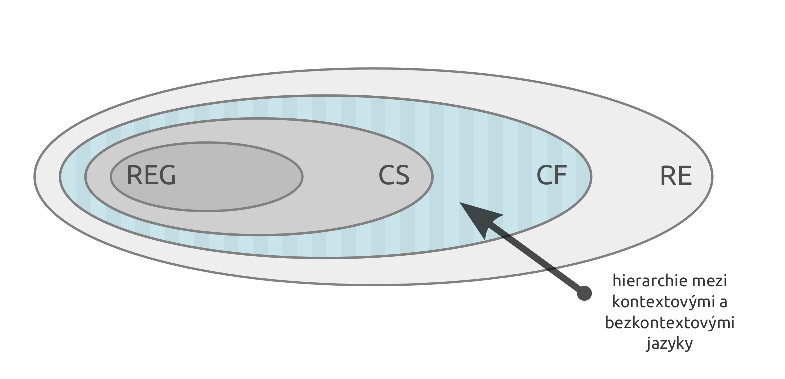
\includegraphics{img/bp_hierarchy01.eps} \bigskip \\
\caption{Znázornění zkoumané oblasti v kontextu Chomského hierarchie.}
\label{obr_chom_hierarchy}
\end{figure}

Mocnosti definovaných modelů se v~rámci Chomského hierarchie nacházejí přibližně mezi kontextovými a bezkontextovými jazyky (obrázek \ref{obr_chom_hierarchy}). Pro bližší zkoumání vztahů mezi jazykovými rodinami zavedu následující označení:

\begin{description*}
\item{\textbf{RE}} je rodina rekurzivně spočetných jazyků,
\item{\textbf{CF}} je rodina kontextových jazyků,
\item{\textbf{CS}} je rodina bezkontextových jazyků,
\item{\textbf{REG}} je rodina regulárních jazyků,

\item{\textbf{${}_n$DP}} je rodina jazyků přijímaných hlubokým zásobníkovým automatem hloubky $n \ge 1$,

\item{\textbf{M}} je rodina jazyků generovaných maticovými gramatikami,
\item{\textbf{P}} je rodina jazyků generovaných programovými gramatikami,
\item{\textbf{S}} je rodina jazyků generovaných stavovými gramatikami,

\end{description*}

$X_{fin}$ indikuje konečný index modelu $X$. Pro modely jazykových rodin \textbf{M}, \textbf{P} a \textbf{S} platí, že vycházejí z~bezkontextové gramatiky a neobsahují $\varepsilon$-pravidla.
Vztahy mezi jazykovými rodinami jsou znázorněné na diagramu \ref{obr_model_hierarchy}. Vycházela jsem z~výsledků v~pracích
Meduny \cite{Meduna:DeepPDA, Meduna:FinitelyDeepPDA, Meduna:StateGrammars}, 
Dassow \cite{Dassow:RegulatedRewriting} a 
Kasai \cite{Kasai:Hierarchy}.


\begin{figure}[ht]
\centering
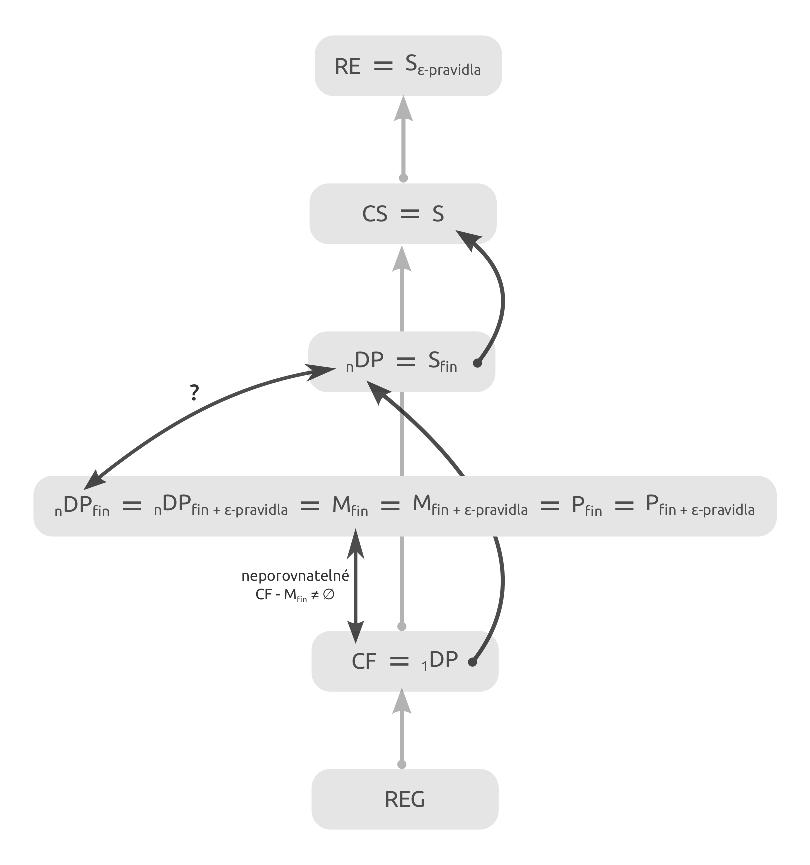
\includegraphics{img/bp_hierarchy02.eps} \bigskip \\
\caption{Grafické srovnání mocností jazykových rodin některých modelů.}
\label{obr_model_hierarchy}
\end{figure}




%=========================================================================
